
%(BEGIN_QUESTION)
% Copyright 2012, Tony R. Kuphaldt, released under the Creative Commons Attribution License (v 1.0)
% This means you may do almost anything with this work of mine, so long as you give me proper credit

Identifiser de to transmitterne som brukes i kaskadereguleringen av væskenivået i ``rundown tank'' i denne ammoniumnitratprosessen, og identifiser hva som skjer med nivået i tanken hvis instrumentluftforsyningen til ammoniumnitrat-flowventilen svikter (dvs. lufttrykket faller til 0 PSI). Anta at flowtransmitteren i sløyfen er direktevirkende og at flowregulatoren er reversvirkende:

$$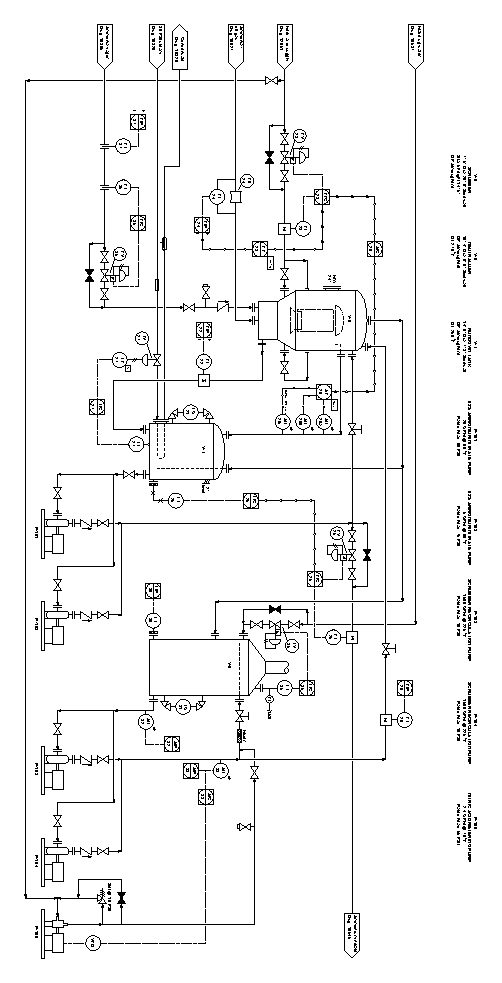
\includegraphics[width=15.5cm]{i01142x01.eps}$$

\underbar{file i01142}
%(END_QUESTION)





%(BEGIN_ANSWER)

{\it 3 poeng for hver korrekt transmitteridentifikasjon, 4 poeng for korrekt konsekvens av luftsvikt.}

\vskip 10pt

Nivåtransmitter for rundown-tank = {\bf LT-26}

\vskip 10pt

Ammoniumnitrat-flowtransmitter = {\bf FT-25}

\vskip 10pt

Hvis instrumentluften svikter, vil nivået i rundown-tanken {\bf øke} fordi FV-25 er fail-closed (FC), og det vil ikke være mulig å få ammoniumnitrat ut av tanken.

%(END_ANSWER)





%(BEGIN_NOTES)


{\bf Denne oppgaven er kun ment for prøver/eksamen, ikke arbeidsark!}.

%(END_NOTES)
